\chapter{Evaluation}
\label{Evaluation}


%\section{Benchmark: File Reading Methods}
%\label{FileReading}
%Three diffrent methods where tested.  The first method utilizes the Java \texttt{Stream} api, to stream the lines of the file. This resulted in a short and intuitiv way of file handeling. The second method uses a \texttt{BufferedReader}, this method was also very easy to set up and reading files by line is a native function. RThe last method was java's implementation of mapped memory. At first the implementation this work would be based on wasn't faster then the other methods, duo to searching in Arrays and String for newline characters. The final implementation iterates over a char buffer provided by the \texttt{MappedByteBuffer} API and retuns a String.
%\begin{figure}[H]
%\centering
%  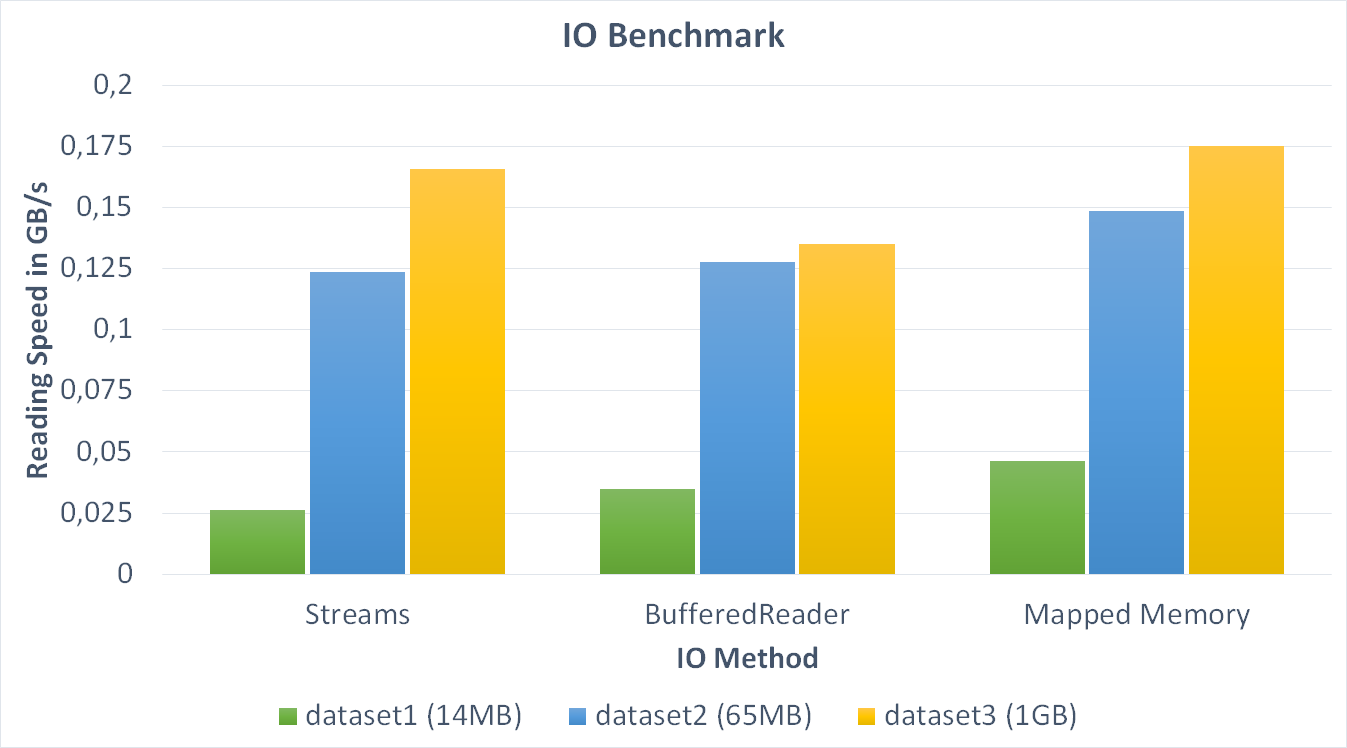
\includegraphics[width=1.0\linewidth]{img/iobench.png}
% \caption{IO Benchmark for File reading in Java}
%  \label{iobench}
%\end{figure}
%The resut of these optimizations can be seen, mapped memory is (not by far) the fastest method, for byte wise input mapped memory was by far the fastest. It can be seen that for the small files from dataset1 the initialization cost is very high compared to the total time taken, but when reading larger files, the initialization seems to be constant and it can be seen that the reading speed converges.